% path to figures directory
\graphicspath{{img/chapter_4/}}

\chapter{Models of neutrino mass and the flavour anomalies}
\label{chapter:neutrino-mass-and-flavour-anomalies}

\section{Introduction}

Taken together, the flavour anomalies paint a picture of new physics interacting
more strongly with the second and third generations of SM fermions, introducing
lepton flavour non-universality and FCNC interactions at energies not
significantly higher than the electroweak scale. Interestingly, many of these
phenomenological motifs arise naturally in radiative models of neutrino mass,
hinting towards the attractive possibility of a common explanation for both
phenomena.

In chapter~\ref{chapter:mv-models}, we presented our model database containing
all minimal tree-level $\Delta L = 2$ models.

Previous work has also considered radiative neutrino mass models whose particle
content addresses $R_{K}$~\cite{Pas:2015hca, Cheung:2016fjo, Cheung:2017efc,
  Cheung:2016frv, Popov:2016fzr}, $R_{D^{(*)}}$~\cite{Deppisch:2016qqd,
  Popov:2016fzr} and $(g-2)_\mu$~\cite{Babu:2010vp, Cheung:2016fjo,
  Cheung:2017efc, Cheung:2016frv, Popov:2016fzr}. In Refs.~\cite{Pas:2015hca,
  Deppisch:2016qqd} the flavour anomalies are explained through two light scalar
or vector leptoquarks whose couplings to the SM Higgs doublet and fermions
prohibit a consistent assignment of lepton number to the leptoquarks such that
the symmetry is respected. Thus $\mathrm{U}(1)_L$ is explicitly broken by two
units and the neutrinos gain mass at the one-loop
level~\cite{AristizabalSierra:2007nf}, apart from the imposition of any
additional symmetries\footnote{Mass generation in Ref.~\cite{Babu:2010vp} occurs
  at the two-loop level because the Yukawa couplings of one of the leptoquarks
  to the left-chiral fermions is turned off.}. A general feature of such models
is that large amounts of fine-tuning are required to suppress the neutrino mass
to the required scale with at least one set of leptoquark--fermion couplings
sizeable enough to explain the anomalies.

\section{A minimal neutrino-mass scenario with $S_{1}$}
\label{sec:ch4-s1-mv}

\begin{figure}[t]
  \centering
  \begin{tikzpicture}
    \begin{feynman}
      \vertex (a) {$\nu$};
      \vertex [right=4em of a] (b);
      \vertex [right=5em of b] (c);
      \vertex [right=5em of c] (d);
      \vertex [right=4em of d] (e) {$\nu$};
      \vertex [above=5em of c] (v);
      \diagram* {
        (a) -- [fermion] (b) -- [anti charged scalar, edge label'=$S_{1}^{a}$] (c) -- [fermion, edge label'=$b$] (d) -- [anti fermion] (e),
        (b) -- [anti fermion, quarter left, edge label=$b$] (v) -- [charged scalar, quarter left, edge label=$S_{1}^{a}$] (d),
        (c) -- [majorana, edge label'=$f$] (v),
      };
    \end{feynman}
  \end{tikzpicture}
  \caption{Two loop neutrino mass generation in the model of
    Ref.~\cite{Angel:2013hla}. For simplicity we consider the case where the
    leptoquark $S_{1}$ couples significantly only to the third generation of
    quarks. At least two flavors of $S_{1}$ are required to meet the neutrino
    data.}
  \label{fig:ch4-neutrinomass}
\end{figure}

In this section we incorporate the BN leptoquark into the two-loop neutrino mass
model developed and studied in detail in Ref.~\cite{Angel:2013hla}. We summarise
the key features of the model below, and point the reader to the original paper
for more detail.

Following Ref.~\cite{Angel:2013hla} we couple the leptoquark $S_{1}$ to the
colour-octet Majorana fermion $f \sim (\mathbf{8}, \mathbf{1}, 0)$ in order to
introduce the lepton-number violating terms $m_f f f$ and
$w_i \bar{d}_i f \phi$. The dimension-9 $\Delta L = 2$ effective operator
$LLQd^cQd^c$ is generated when the heavy fields $f$ and $\phi$ are integrated
out. The neutrino mass is proportional to the product of down-type quark mass
matrices, which is dominated by the bottom quark mass. We do not consider the
case where a strong hierarchy in the $w_i$ undermines this dominance, and thus
only the coupling to the third generation of quarks ($w_3$) is important for the
neutrino mass generation. For this reason we set $w_{1,2} = 0$ to simplify the
calculation of the neutrino mass. In this limit the neutrino mass matrix will
have unit rank and an additional generation of the leptoquark $\phi$ is needed
to satisfy current oscillation data. Replacing $S_{1}$ with
$S_{1}^{a} = (S^{1}_1, S_1^{2})$ in Eq.~\eqref{eq:ch3-Lagra}, small neutrino
masses are generated through the two-loop graph shown in
Fig.~\ref{fig:ch4-neutrinomass} and the neutrino mass is given by
\begin{equation}
  \label{eq:ch4-massformula}
  M_{ij} \approx 4\frac{m_f
    m_b^2}{(2\pi)^8} \sum_{a, b}^2 (x_{i3a} w_{3a}) I_{ab}
  (x_{j3b} w_{3b}),
\end{equation}
where $\mathbf{I}$ is the matrix of loop integrals in the leptoquark-generation
space whose explicit form can be found in Ref.~\cite{Angel:2013hla}. This
expression for the mass matrix can be solved for the $x_{i3a}$ through the
Casas--Ibarra procedure~\cite{Casas:2001sr} to give
\begin{equation}
  \label{eq:ch4-ci}
  x_{i3a} = \frac{(2\pi)^4}{2w_{3a}m_b\sqrt{m_f}} U^*_{ij} [\tilde{\mathbf{M}}^{1/2}]_{jk} R_{kb} [\tilde{\mathbf{I}}^{-1/2}\mathbf{S}]_{ba},
\end{equation}
where tildes denote real and positive diagonal matrices and $\mathbf{S}$
diagonalizes the matrix $\mathbf{I}$. We use the best-fit values from the NuFIT
collaboration for the neutrino mixing angles and mass-squared
differences~\cite{Esteban:2016qun, nufitweb}:
\begin{equation}
  \begin{aligned}
    \sin^2 \theta_{12} &= 0.306,   & \Delta m_{21}^2 &= 7.50 \cdot 10^{-5} \text{ eV}^{2},\\
    \sin^2 \theta_{13} &= 0.02166, & \Delta m_{31}^2 &= 2.524 \cdot 10^{-3} \text{ eV}^{2} \text{ (NO)},\\
    \sin^2 \theta_{23} &= 0.441 \text{ (NO)},   & \Delta m_{32}^2 &= -2.514 \cdot 10^{-3} \text{ eV}^{2} \text{ (IO)},\\
    \sin^2 \theta_{23} &= 0.587 \text{ (IO)}.
  \end{aligned}
\end{equation}
The mass-squared differences fix the elements of $\tilde{\mathbf{M}}$, since the
lightest neutrino in this model is almost massless. In the cases of normal and
inverted neutrino mass hierarchy,
\begin{equation} \label{eq:ch4-r}
  \mathbf{R}^{\textsc{NO}} = \begin{pmatrix} 0 & 0\\ \cos\theta & -\sin\theta \\ \sin\theta & \cos\theta\end{pmatrix}, \quad
  \mathbf{R}^{\textsc{IO}} = \begin{pmatrix} \cos\theta & -\sin\theta \\ \sin\theta & \cos\theta \\ 0 & 0 \\\end{pmatrix},
\end{equation}
and $\theta \in \mathbb{C}$ parameterizes the leptoquark--fermion Yukawa
couplings through Eq.~\eqref{eq:ci} in such a way that the correct pattern of
neutrino masses and mixings is produced. Here we consider the region of
parameter space where $m_{S_{1}^2} , m_{f} \gg m_{S_{1}^1}$ so that $S_1^{1}$
comes to be identified as the BN leptoquark, while $S_{1}^2$ and $f$ are
effectively divorced from the flavor anomalies. For this reason we refer to
$S_{1}^{1}$ simply as $S_{1}$ and suppress the leptoquark-flavour indices for
the remainder of the discussion unless a distinction is necessary. The limit
$m_{S_{1}^1} \ll m_{S_{1}^{2}}$ also allows for a simplification in the matrix
product $\tilde{\mathbf{I}}^{-1/2}\mathbf{S}$ featuring in Eq.~\eqref{eq:ch4-ci}:
\begin{equation}
  \tilde{\mathbf{I}}^{-1/2}\mathbf{S} \approx I_{11}^{-1/2} \begin{pmatrix} -i & i/\epsilon \\ 1 & \epsilon \\ \end{pmatrix},
\end{equation}
where $\epsilon \equiv I_{12}/I_{11} \ll 1$. This flavor structure implies that its
contribution to neutrino mixing is small, and thus the PMNS parameters are
principally determined by the Yukawa couplings $x_{i3a}$. We exploit this
relative insensitivity to $m_f$ and $m_{S_{1}^{2}}$ to simplify our analysis in
the following.

The decoupling of $f$ and $S_{1}^{2}$ from the relevant flavor physics makes
$w_3$ an effectively free parameter that acts as a lepton-flavor-blind scaling
factor on the couplings of the leptoquark to the third generation of quarks,
while $\theta$ governs their relative sizes for a given leptoquark flavor. We
plot the $x_{i3}$ against real $\theta$ values in Fig.~\ref{fig:ch4-xi3plot} for
the mass choices $m_f = 25 \text{ TeV}$, $m_{S_{1}^{2}} = 20 \text{ TeV}$ and
$m_{S_{1}^{1}} = 4 \text{ TeV}$ with fixed $w_3 = 0.003$. Both the normal and
inverted hierarchies are considered.

\begin{figure}[t]
  \centering%
  \begin{minipage}[t]{0.45\linewidth}
    \centering 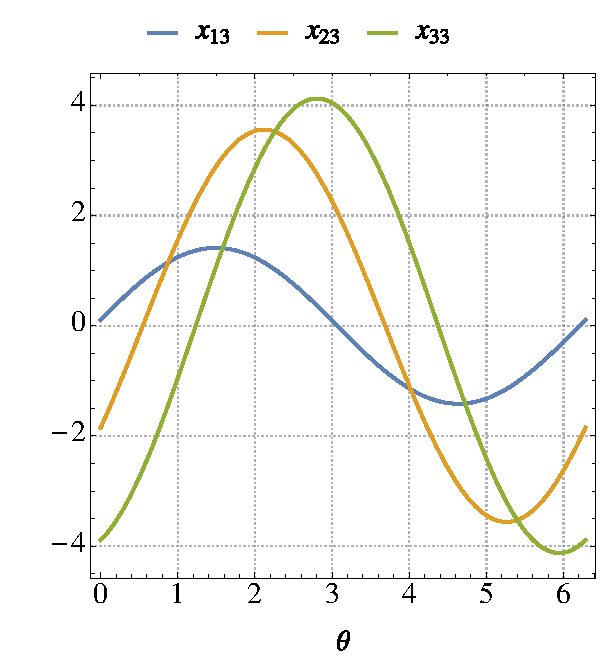
\includegraphics[scale=0.55]{xi3Plot.pdf}
    \subcaption{Normal neutrino mass hierarchy.}
    \label{fig:noxi3plot}
  \end{minipage}
  \hfill
  \begin{minipage}[t]{0.45\linewidth}
    \centering 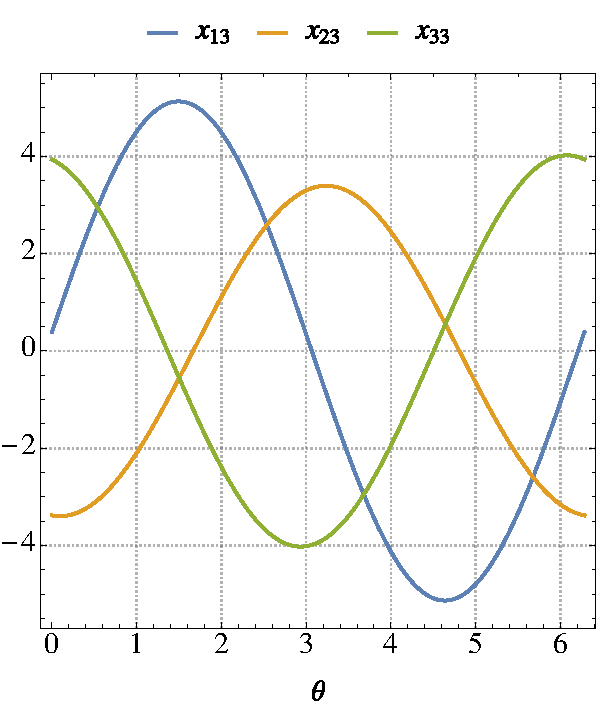
\includegraphics[scale=0.51]{xi3PlotIO.pdf}
    \subcaption{Inverted neutrino mass hierarchy.}
    \label{fig:ioxi3plot}
  \end{minipage}
  \caption{Plots of the relative sizes of the couplings of the leptoquark
    $\phi_1$ to the bottom quark and the $i$th neutrino flavor against $\theta$,
    the Casas--Ibarra parameter, for $m_f = 25 \text{ TeV}$, $m_{\phi_2} = 20
    \text{ TeV}$, $m_{\phi_1} = 4 \text{ TeV}$ and $w_3 = 0.003$. We only
    consider the case $\theta \in \mathbb{R}$ here.}
  \label{fig:ch4-xi3plot}
\end{figure}

Both Fig.~\ref{fig:ch4-xi3plot} and Eq.~\eqref{eq:ch4-ci} indicate that, with the
inclusion of neutrino mass, the couplings to the electron and electron-neutrino
cannot be turned off \textit{ad libitum}. Even a small electron coupling $z_{13}
\neq 0$ can generate dangerous contributions to muon--electron conversion in
nuclei in the presence of $z_{23} \neq 0$, necessary for the model to alleviate
the tensions in the $b \to s$ transition. We plot the current limit from
muon--electron conversion experiments in gold nuclei $\text{Br}(\mu
\ce{^{197}_{79}}\text{Au} \to e \ce{^{197}_{79}}\text{Au}) < 7.0 \cdot
10^{-13}$~\cite{Olive:2016xmw} against $\theta$ and $w_3$ in
Fig.~\ref{fig:ch4-muNeN} for both the normal and inverted hierarchies and a range of
masses $m_{\phi_1}$. The prospective limit from the COMET experiment: $\text{Br}
\sim 10^{-16}$~\cite{Kurup:2011zza}, is also shown. A fit to the neutrino
oscillation data while respecting measurements of muon--electron conversion
implies a fine-tuning in $\theta$---or, equivalently, $z_{31}$---to arrange
$|z_{31}| \ll |z_{33}|$, pushing the model into a very specific region of
parameter space. The required $x_{31} \approx 0$ can be arranged with $\theta
\approx 3.08 \pm n\pi$, fixing the ratio $x_{33}/x_{32} = 1.96$ for the normal
neutrino mass hierarchy, and $x_{33}/x_{32} = -0.85$ for the inverted hierarchy.
Comparison with Fig.~\ref{fig:ch3-x33x32rat}, however, indicates that neither of the
aforementioned ratios can allow large contributions to $R_{K^{(*)}}$ in the
correct direction, although the inverted hierarchy does slightly better than the
normal mass ordering. This makes a combined explanation of the $b \to s$
anomalies and neutrino mass in this model problematic. If, instead, one required
that this model explain $R_{D^{(*)}}$, $(g-2)_\mu$ and neutrino mass, the values
of $x_{33}$ required are compatible with both the normal and inverted
hierarchies, and the model remains agnostic with respect to its preference.

\begin{figure}[t]
  \centering
  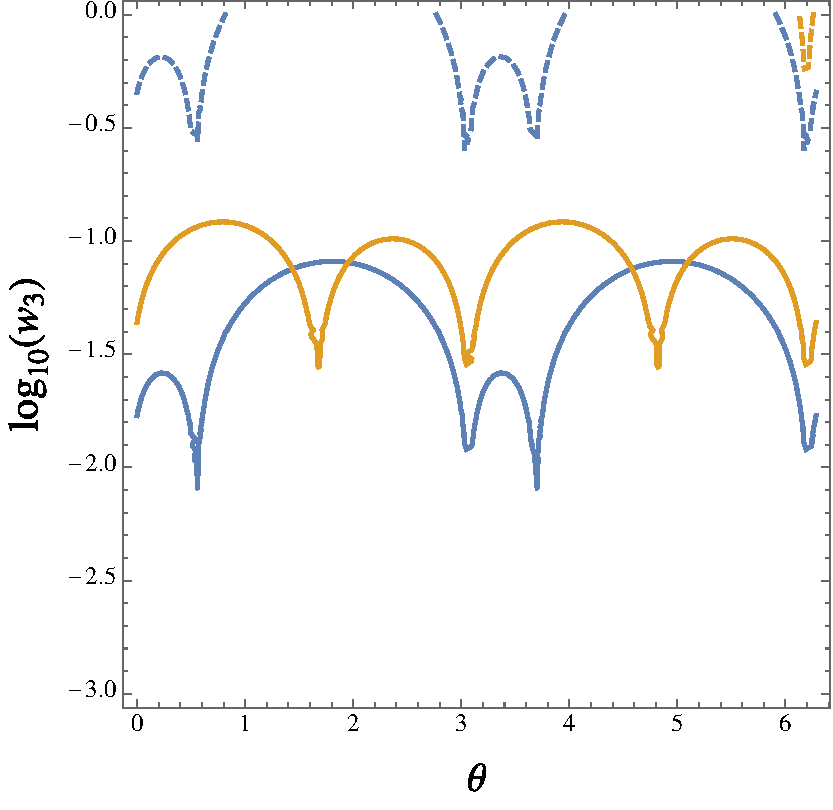
\includegraphics[scale=0.45]{muNeN}
  \caption{The figure shows the current (solid) and
    expected~\cite{Kurup:2011zza} (dashed) limits from muon--electron conversion
    in nuclei in the $\theta$--$w_3$ plane for normal mass ordering (blue) and
    inverted ordering (orange). The region below each curve is ruled out. The
    dips at $\theta \approx 3.08$ and $\theta \approx 6.22$ stretch to negative
    infinity. Aside from accidental cancellation, the values $\theta \approx
    3.08, 6.22$ ensure that the coupling to the electron vanishes. Only real
    values of $\theta$ are considered.}
  \label{fig:ch4-muNeN}
\end{figure}

\section{A non-minimal model: $S_{1}$ and $S_{3}$}
\label{sec:ch4-non-minimal}

\lipsum[1]

\subsection{The model}
\lipsum[1]

\subsection{Neutrino mass}
\lipsum[1]

\subsection{Flavour anomalies}
\lipsum[1]

\subsection{Contraints}
\lipsum[1]

\subsubsection{Collider bounds}
\lipsum[1]

\subsubsection{Fermion mixing}
\lipsum[1]

\subsubsection{Other constraints}
\lipsum[1]

\subsection{Results and discussion}
\lipsum[1]

\section{Conclusions}
\lipsum[1]
